% Created by tikzDevice version 0.12.6 on 2026-03-25 10:37:05
% !TEX encoding = UTF-8 Unicode
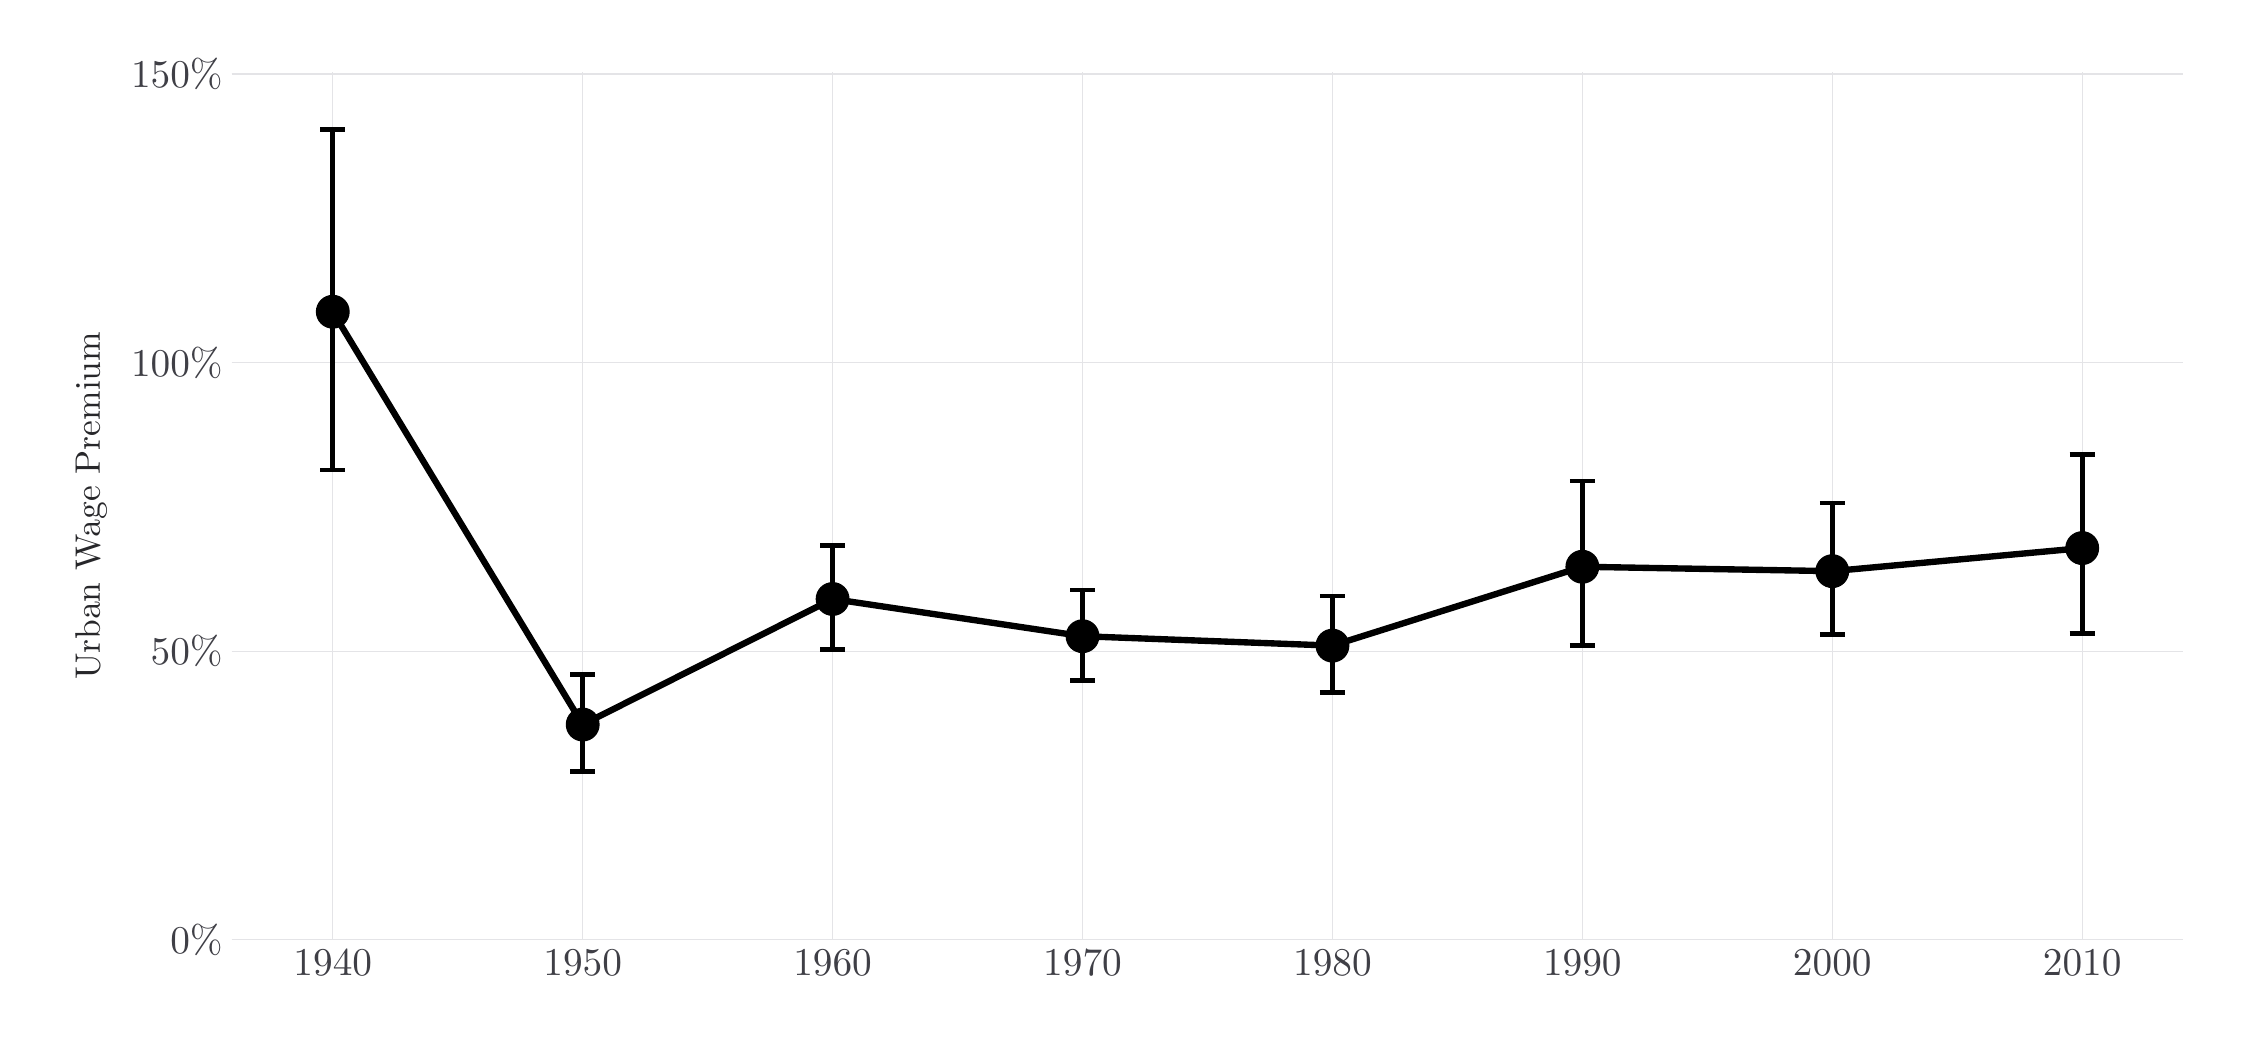
\begin{tikzpicture}[x=1pt,y=1pt]
\definecolor{fillColor}{RGB}{255,255,255}
\path[use as bounding box,fill=fillColor] (0,0) rectangle (794.97,361.35);
\begin{scope}
\path[clip] (  0.00,  0.00) rectangle (794.97,361.35);
\definecolor{drawColor}{RGB}{255,255,255}

\path[draw=drawColor,line width= 0.8pt,line join=round,line cap=round,fill=fillColor] ( -0.00,  0.00) rectangle (794.97,361.35);
\end{scope}
\begin{scope}
\path[clip] ( 73.68, 31.76) rectangle (778.97,345.35);
\definecolor{drawColor}{RGB}{255,255,255}
\definecolor{fillColor}{RGB}{255,255,255}

\path[draw=drawColor,line width= 0.8pt,line join=round,line cap=round,fill=fillColor] ( 73.68, 31.76) rectangle (778.97,345.35);
\definecolor{drawColor}{RGB}{228,228,231}

\path[draw=drawColor,line width= 0.4pt,line join=round] ( 73.68, 31.76) --
	(778.97, 31.76);

\path[draw=drawColor,line width= 0.4pt,line join=round] ( 73.68,136.04) --
	(778.97,136.04);

\path[draw=drawColor,line width= 0.4pt,line join=round] ( 73.68,240.33) --
	(778.97,240.33);

\path[draw=drawColor,line width= 0.4pt,line join=round] ( 73.68,344.61) --
	(778.97,344.61);

\path[draw=drawColor,line width= 0.4pt,line join=round] (110.25, 31.76) --
	(110.25,345.35);

\path[draw=drawColor,line width= 0.4pt,line join=round] (200.56, 31.76) --
	(200.56,345.35);

\path[draw=drawColor,line width= 0.4pt,line join=round] (290.86, 31.76) --
	(290.86,345.35);

\path[draw=drawColor,line width= 0.4pt,line join=round] (381.17, 31.76) --
	(381.17,345.35);

\path[draw=drawColor,line width= 0.4pt,line join=round] (471.48, 31.76) --
	(471.48,345.35);

\path[draw=drawColor,line width= 0.4pt,line join=round] (561.78, 31.76) --
	(561.78,345.35);

\path[draw=drawColor,line width= 0.4pt,line join=round] (652.09, 31.76) --
	(652.09,345.35);

\path[draw=drawColor,line width= 0.4pt,line join=round] (742.40, 31.76) --
	(742.40,345.35);
\definecolor{drawColor}{RGB}{0,0,0}

\path[draw=drawColor,line width= 2.3pt,line join=round] (110.25,258.70) --
	(200.56,109.53) --
	(290.86,154.90) --
	(381.17,141.45) --
	(471.48,138.05) --
	(561.78,166.55) --
	(652.09,164.96) --
	(742.40,173.29);

\path[draw=drawColor,line width= 1.7pt,line join=round] (105.73,324.49) --
	(114.77,324.49);

\path[draw=drawColor,line width= 1.7pt,line join=round] (110.25,324.49) --
	(110.25,201.54);

\path[draw=drawColor,line width= 1.7pt,line join=round] (105.73,201.54) --
	(114.77,201.54);

\path[draw=drawColor,line width= 1.7pt,line join=round] (196.04,127.59) --
	(205.07,127.59);

\path[draw=drawColor,line width= 1.7pt,line join=round] (200.56,127.59) --
	(200.56, 92.54);

\path[draw=drawColor,line width= 1.7pt,line join=round] (196.04, 92.54) --
	(205.07, 92.54);

\path[draw=drawColor,line width= 1.7pt,line join=round] (286.35,174.15) --
	(295.38,174.15);

\path[draw=drawColor,line width= 1.7pt,line join=round] (290.86,174.15) --
	(290.86,136.71);

\path[draw=drawColor,line width= 1.7pt,line join=round] (286.35,136.71) --
	(295.38,136.71);

\path[draw=drawColor,line width= 1.7pt,line join=round] (376.65,158.16) --
	(385.68,158.16);

\path[draw=drawColor,line width= 1.7pt,line join=round] (381.17,158.16) --
	(381.17,125.57);

\path[draw=drawColor,line width= 1.7pt,line join=round] (376.65,125.57) --
	(385.68,125.57);

\path[draw=drawColor,line width= 1.7pt,line join=round] (466.96,156.02) --
	(475.99,156.02);

\path[draw=drawColor,line width= 1.7pt,line join=round] (471.48,156.02) --
	(471.48,121.06);

\path[draw=drawColor,line width= 1.7pt,line join=round] (466.96,121.06) --
	(475.99,121.06);

\path[draw=drawColor,line width= 1.7pt,line join=round] (557.27,197.54) --
	(566.30,197.54);

\path[draw=drawColor,line width= 1.7pt,line join=round] (561.78,197.54) --
	(561.78,138.13);

\path[draw=drawColor,line width= 1.7pt,line join=round] (557.27,138.13) --
	(566.30,138.13);

\path[draw=drawColor,line width= 1.7pt,line join=round] (647.57,189.64) --
	(656.60,189.64);

\path[draw=drawColor,line width= 1.7pt,line join=round] (652.09,189.64) --
	(652.09,141.95);

\path[draw=drawColor,line width= 1.7pt,line join=round] (647.57,141.95) --
	(656.60,141.95);

\path[draw=drawColor,line width= 1.7pt,line join=round] (737.88,207.06) --
	(746.91,207.06);

\path[draw=drawColor,line width= 1.7pt,line join=round] (742.40,207.06) --
	(742.40,142.48);

\path[draw=drawColor,line width= 1.7pt,line join=round] (737.88,142.48) --
	(746.91,142.48);
\definecolor{fillColor}{RGB}{0,0,0}

\path[draw=drawColor,line width= 0.5pt,line join=round,line cap=round,fill=fillColor] (110.25,258.70) circle (  5.87);

\path[draw=drawColor,line width= 0.5pt,line join=round,line cap=round,fill=fillColor] (200.56,109.53) circle (  5.87);

\path[draw=drawColor,line width= 0.5pt,line join=round,line cap=round,fill=fillColor] (290.86,154.90) circle (  5.87);

\path[draw=drawColor,line width= 0.5pt,line join=round,line cap=round,fill=fillColor] (381.17,141.45) circle (  5.87);

\path[draw=drawColor,line width= 0.5pt,line join=round,line cap=round,fill=fillColor] (471.48,138.05) circle (  5.87);

\path[draw=drawColor,line width= 0.5pt,line join=round,line cap=round,fill=fillColor] (561.78,166.55) circle (  5.87);

\path[draw=drawColor,line width= 0.5pt,line join=round,line cap=round,fill=fillColor] (652.09,164.96) circle (  5.87);

\path[draw=drawColor,line width= 0.5pt,line join=round,line cap=round,fill=fillColor] (742.40,173.29) circle (  5.87);
\end{scope}
\begin{scope}
\path[clip] (  0.00,  0.00) rectangle (794.97,361.35);
\definecolor{drawColor}{RGB}{63,63,70}

\node[text=drawColor,anchor=base east,inner sep=0pt, outer sep=0pt, scale=  1.42] at ( 70.48, 26.86) {0\%};

\node[text=drawColor,anchor=base east,inner sep=0pt, outer sep=0pt, scale=  1.42] at ( 70.48,131.15) {50\%};

\node[text=drawColor,anchor=base east,inner sep=0pt, outer sep=0pt, scale=  1.42] at ( 70.48,235.43) {100\%};

\node[text=drawColor,anchor=base east,inner sep=0pt, outer sep=0pt, scale=  1.42] at ( 70.48,339.72) {150\%};
\end{scope}
\begin{scope}
\path[clip] (  0.00,  0.00) rectangle (794.97,361.35);
\definecolor{drawColor}{RGB}{63,63,70}

\node[text=drawColor,anchor=base,inner sep=0pt, outer sep=0pt, scale=  1.42] at (110.25, 18.76) {1940};

\node[text=drawColor,anchor=base,inner sep=0pt, outer sep=0pt, scale=  1.42] at (200.56, 18.76) {1950};

\node[text=drawColor,anchor=base,inner sep=0pt, outer sep=0pt, scale=  1.42] at (290.86, 18.76) {1960};

\node[text=drawColor,anchor=base,inner sep=0pt, outer sep=0pt, scale=  1.42] at (381.17, 18.76) {1970};

\node[text=drawColor,anchor=base,inner sep=0pt, outer sep=0pt, scale=  1.42] at (471.48, 18.76) {1980};

\node[text=drawColor,anchor=base,inner sep=0pt, outer sep=0pt, scale=  1.42] at (561.78, 18.76) {1990};

\node[text=drawColor,anchor=base,inner sep=0pt, outer sep=0pt, scale=  1.42] at (652.09, 18.76) {2000};

\node[text=drawColor,anchor=base,inner sep=0pt, outer sep=0pt, scale=  1.42] at (742.40, 18.76) {2010};
\end{scope}
\begin{scope}
\path[clip] (  0.00,  0.00) rectangle (794.97,361.35);
\definecolor{drawColor}{RGB}{39,39,42}

\node[text=drawColor,rotate= 90.00,anchor=base,inner sep=0pt, outer sep=0pt, scale=  1.28] at ( 26.06,188.55) {Urban Wage Premium};
\end{scope}
\end{tikzpicture}
